\chapter{Overview}
\label{sct:overview}

CernVM currently supports images for VirtualBox, VMware, Xen, KVM and Microsoft Hyper-V hypervisors, each new release of a CernVM image needs to be 
thoroughly tested on each supported platform and hypervisor. The \cernvmreleasetesting\ project is designed to meet this requirement by providing an 
automated testing environment for CernVM images, which will install and configure CernVM images, run the set of tests and report the results on a web
interface.

The intent of this document is to provided a step-by-step guide on setting up an entire \cernvmreleasetesting\ infrastructure, including instructions
on how to set up and configure test clients, the main server running the web interface and database, as well as writing and executing tests. If you are
new to release testing and want a document to guide you through the entire process of setting up a working \cernvmreleasetesting\ infrastructure,
then this guide for you.

All the code needed to setup the entire \releasetesting\ infrastructure for CernVM image testing, is located at the 
\cernvmreleasetesting\ Google Code project page\cite{GCreleasetesting} including this document and all other documentation. 

While this document is not intended to be a replacement for the reference manual, the following is a brief description of the \releasetesting\ infrastructure 
including an introduction to the core component, \amdtapper\cite{tapper}. Figure~\ref{fig:architecture} consists of a diagram outlining the
\indexed{\tapper~Architecture}, which consists of test clients and a server, the server is what controls the test clients, gathers 
results, and then displays the results through a web interface.\newline

\begin{figure}[!hbp]
	\begin{center}
		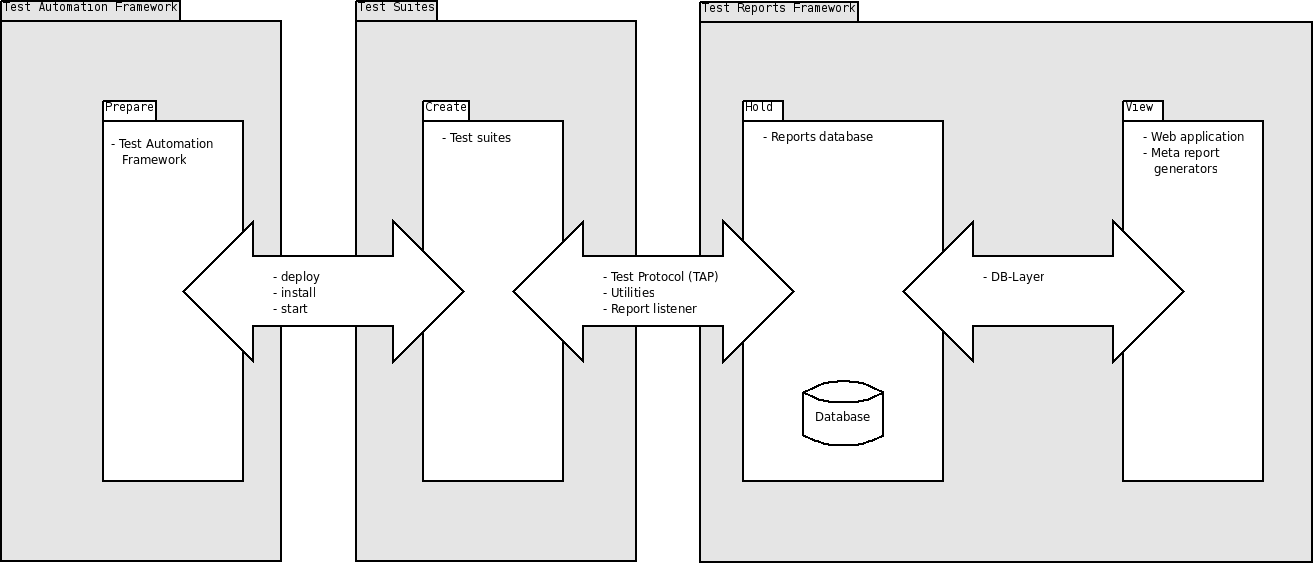
\includegraphics[scale=0.25]{img/tapper_architecture_overview.png}
	\end{center}
	\caption{Overview of the \tapper architecture}
	\label{fig:architecture}
\end{figure}

The components of the \releasetesting~Framework are listed in Table~\ref{tbl:components}. 

\begin{table}
  \begin{center}

    \begin{tabularx}{\linewidth}{l|X}
      {\bf\centering \releasetesting component name} & {\bf\centering Description} \\\hline
%        \texttt{Agent} & Communicates with service insances and requests a job to execute. Upon receiving the job downloads the input 
%                         files, executes the job, uploads job output files and reports that the job execution is finished. \\
%        \texttt{Generic Job and Storage Manager} & Distributes jobs from the internal queue to Agents for execution, provides space for storing 
%                                                   the job output   \\
%        \texttt{AliEn Job Manager} & Retrieves jobs from the central task queue of \indexed{AliEn} Grid \cite{alien} and sends them to 
%                                     Agents for execution \\
%        \texttt{AliEn Storage Manager} & Uploads the output of AliEn jobs executed by Agents and finalizes the job status in AliEn Grid.  \\
%        \texttt{PanDA Storage Manager} & Uploads the output of \indexed{PanDA} \cite{panda} jobs executed by Agents and finalizes the job status in PanDA Grid  \\
    \end{tabularx}  
  \end{center}

  \caption{List of \releasetesting and \amdtapper components}

  \label{tbl:components}
\end{table}
